% =============================================================================
% Bridging Semantic and Relational Spaces: A Dual-Layer Architecture
% for Neuro-Symbolic Agent Memory
% =============================================================================
% CEUR-ART Single-Column Format — Discussion Paper (V4 Final)
% =============================================================================

\documentclass{ceurart}

%% Fix overfull hboxes (per official CEUR-ART sample)
\sloppy

%% TikZ for native diagrams (no \includegraphics)
\usepackage{tikz}
\usetikzlibrary{shapes.geometric,arrows.meta,positioning,fit,shadows,backgrounds,calc}

%% Algorithms
\usepackage{algorithm}
\usepackage{algpseudocode}

%% URL support
\usepackage{url}

%% amsmath, graphicx, booktabs, hyperref loaded automatically by ceurart.cls

% =============================================================================
% Front Matter
% =============================================================================

\begin{document}

\copyrightyear{2026}
\copyrightclause{Copyright for this paper by its authors.
  Use permitted under Creative Commons License Attribution 4.0
  International (CC BY 4.0).}

\conference{Workshop on Graphs Across AI, 2026}

\title{Bridging Semantic and Relational Spaces: A Dual-Layer Architecture
  for Neuro-Symbolic Agent Memory}

\author[1]{Mustafa Arslan}[%
  email=mustafarslan35@gmail.com
]
\address[1]{Independent Researcher, Istanbul, Turkey}

% -----------------------------------------------------------------------------
% Abstract
% -----------------------------------------------------------------------------
\begin{abstract}
Large Language Models are fundamentally constrained by the quadratic cost of
self-attention and the empirically observed degradation of reasoning as context
windows expand, a failure mode known as the ``Lost in the Middle'' phenomenon.
Existing Retrieval-Augmented Generation (RAG) architectures treat agent memory
as an unstructured bag of embeddings, leading to \emph{Vector Haze}: the
retrieval of semantically similar yet episodically disconnected facts that
confuse the agent rather than aid it. This paper proposes a dual-layer
Cognitive Operating System that redefines memory as a managed, structured
resource. \textbf{Layer~1}, the Micro-Graph Kernel (Aeon), formalizes episodic
memory as a neuro-symbolic Directed Acyclic Graph (DAG) with formally defined
temporal, causal, and referential edge families, and introduces the
\emph{Semantic Lookaside Buffer} (SLB), a predictive caching mechanism that
exploits conversational locality to achieve $O(K)$ retrieval complexity against
a buffer of $K$ centroids, bypassing the $O(\log N)$ cost of global index
traversal. \textbf{Layer~2}, the Macro-Graph Router (PandoraLM), implements a
dual-process cognitive router inspired by Kahneman's \emph{Thinking, Fast and
Slow}, dynamically selecting between rapid vector search and deliberate
multi-hop graph reasoning. The paper provides formal complexity analyses for
each retrieval mode, demonstrates through a concrete scenario how AST-aware
graph retrieval resolves polymorphic inheritance chains that defeat flat
chunking, details a deterministic ReBAC security model that eliminates
Time-of-Check to Time-of-Use vulnerabilities in agentic pipelines, and
proposes a biologically inspired \emph{Memory Consolidation} process (the
migration of transient episodic traces into the persistent spatial index,
termed the \emph{Memory Palace}) with explicit graph-pruning invariants for
bridging episodic traces with enterprise knowledge graphs.
\end{abstract}

\begin{keywords}
  Neuro-symbolic AI \sep
  Agent memory \sep
  Graph-based retrieval \sep
  Cognitive routing \sep
  Episodic DAG \sep
  Semantic caching
\end{keywords}

\maketitle

% =============================================================================
% Section 1: Introduction
% =============================================================================
\section{Introduction: Navigating the Vector Haze}

The current paradigm of Retrieval-Augmented Generation (RAG) is encountering a
structural ceiling. While Large Language Models (LLMs) have demonstrated
remarkable generative capabilities, their capacity to maintain a coherent
``self'' over thousands of interaction turns is fundamentally limited by how
they access information. Standard retrieval mechanisms, here characterized
as \emph{Flat RAG}, treat an agent's history as a featureless plane: a ``bag
of vectors'' where every query is an independent event, disconnected from the
temporal and causal lineage of the task~\cite{karpukhin2020dense}.

This statelessness leads to a phenomenon defined herein as \textbf{Vector
Haze}\footnote{The
complete Aeon system, including the high-performance kernel implementation
with hardware-specific optimizations (e.g., SIMD-accelerated search,
zero-copy memory bridges), is described in the full technical paper
(arXiv:2601.15311)~\cite{arslan2026aeon}. This discussion paper explicitly
isolates the neuro-symbolic graph topology and proposes its
application-layer orchestration.}: the retrieval of semantically similar but
episodically disjointed facts that confuse the agent rather than aid
it~\cite{arslan2026aeon}. In long-horizon, high-stakes technical
environments, Vector Haze manifests as the agent losing the ``narrative arc''
of a project, failing to remember why a specific architectural decision was
made three sessions ago, or hallucinating outdated API signatures because they
appear semantically ``closer'' in a high-dimensional
space~\cite{liu2023lost}. Research on context utilization has confirmed that
LLM reasoning degrades significantly when relevant information is buried
within an expanded context window, further underscoring that models cannot
simply ``attend to everything'' but must \emph{structurally select}
context~\cite{liu2023lost}.

This failure is not merely an engineering inconvenience; it is a theoretical
limitation of treating similarity as the sole proxy for relevance. Consider a
software debugging session: a code snippet from a different project may be
semantically identical to the current file (sharing function names, variable
patterns, and docstring vocabulary) yet bear zero causal relevance to the bug at
hand. Without structural edges that encode \emph{how} and \emph{why} that
snippet entered the agent's history, the retrieval system cannot distinguish it
from the genuinely relevant code. As recent work on continuum memory has
argued, memory for autonomous agents must be a \emph{continuously evolving
substrate} that mutates and consolidates, rather than a stateless lookup table
reconstructed from scratch at every turn~\cite{zhang2026continuum}.

This paper proposes a paradigm shift: the treatment of agent memory as a resource
managed by a neuro-symbolic \textbf{Cognitive Operating System}. The proposed
architecture is composed of two synergistic layers:

\begin{itemize}
  \item \textbf{Layer 1, the Micro-Graph Kernel (Aeon):} Formalizes episodic
    memory as a Directed Acyclic Graph (DAG) with typed edges preserving
    temporal and causal structure~\cite{arslan2026aeon}. It introduces the
    \emph{Semantic Lookaside Buffer} (SLB), a predictive caching mechanism
    that exploits conversational locality to bypass retrieval latency.
  \item \textbf{Layer 2, the Macro-Graph Router (PandoraLM):} Implements a
    dual-process cognitive router inspired by Kahneman's \emph{Thinking, Fast
    and Slow}~\cite{kahneman2011}, dynamically determining when to rely on
    rapid System~1 vector retrieval versus slow, deliberate System~2 graph
    reasoning over global knowledge structures and structural codebase
    ASTs~\cite{cognitiverouting2025}.
\end{itemize}

By bridging high-performance graph topologies with adaptive cognitive routing,
this dual-layer OS provides a deterministic navigational overlay to
probabilistic vector spaces. Table~\ref{tab:retrieval} summarizes the
landscape of retrieval paradigms this architecture bridges.

\begin{table}[t]
  \caption{Comparison of Retrieval Paradigms for Agent Memory}
  \label{tab:retrieval}
  \begin{tabular}{llll}
    \toprule
    \textbf{Type} & \textbf{Representation} & \textbf{Navigation} & \textbf{Fidelity} \\
    \midrule
    Flat Vector      & Bag of Embeddings       & Distance (ANN)       & Low (Vector Haze) \\
    Episodic DAG     & Causal/Temporal Nodes   & Edge Traversal       & High (Causal) \\
    Knowledge Graph  & Relational Entities     & Multi-hop Reasoning  & High (Thematic) \\
    AST Map          & Structural Code Units   & Hierarchical Nav.    & Precise (Logical) \\
    \bottomrule
  \end{tabular}
\end{table}

The contributions of this paper are threefold: (1) a formal specification of
the Trace episodic DAG with typed edge families and complexity analysis of
graph-based versus vector-based retrieval; (2) the Semantic Lookaside Buffer
with theoretical grounding in the Semantic Inertia hypothesis and an explicit
$O(K)$ versus $O(\log N)$ complexity comparison; and (3) a dual-process
cognitive routing architecture with concrete failure-mode analysis for
polymorphic code resolution, deterministic ReBAC security guarantees, and a
graph-pruning consolidation algorithm with formally stated invariants.

The remainder of this paper is organized as follows. Section~\ref{sec:trace}
formalizes the Trace as an episodic graph memory. Section~\ref{sec:slb}
presents the Semantic Lookaside Buffer as a predictive graph cache.
Section~\ref{sec:routing} details the cognitive routing and enterprise graph
integration of Layer~2. Section~\ref{sec:discussion} discusses the synergy
between layers and proposes a ``Dreaming'' consolidation process, and
Section~\ref{sec:conclusion} concludes with open questions.


% =============================================================================
% Section 2: The Trace — Episodic Graph Memory
% =============================================================================
\section{The Trace: Episodic Memory as a Directed Acyclic Graph}
\label{sec:trace}

The transition from flat vector stores to graph-based memory is necessitated by
the inherent structure of human and agentic experience. Human memory is not a
random-access lookup table; it is a continuously evolving substrate that relies
on time and causality as scaffolds for recall~\cite{zhang2026continuum}.
Replicating this capacity in AI agents necessitates a topological model of
experience that preserves relational dependencies~\cite{graphagentmem2025}.

\subsection{Formal Graph Definition}

The \emph{Trace} is the episodic memory subsystem of the Aeon Micro-Graph
Kernel. It is structured as a Directed Acyclic Graph
$G = (V, E)$~\cite{arslan2026aeon}, where the vertex set $V$ is partitioned
into three disjoint subsets:

\begin{equation}
  V = V_{\text{user}} \cup V_{\text{system}} \cup V_{\text{concept}}, \quad
  V_{\text{user}} \cap V_{\text{system}} = \emptyset, \quad
  V_{\text{user}} \cap V_{\text{concept}} = \emptyset, \quad
  V_{\text{system}} \cap V_{\text{concept}} = \emptyset
\end{equation}

\noindent The three vertex partitions are defined as follows. $V_{\text{user}}$
contains human input events (utterances, commands, and feedback).
$V_{\text{system}}$ contains agent-generated responses (answers, actions, and
tool invocations). $V_{\text{concept}}$ contains abstract semantic cluster
nodes that serve as stable reference anchors in the embedding space.

Each node $v \in V$ carries a composite payload:
\begin{equation}
  v = (\mathbf{e}_v, \; t_v, \; m_v)
\end{equation}
\noindent where $\mathbf{e}_v \in \mathbb{R}^d$ is a dense embedding vector
encoding semantic content, $t_v \in \mathbb{R}^+$ is a monotonically
increasing timestamp, and $m_v$ is a metadata record containing session
identifiers, tool-call traces, and token counts. This hybrid design (neural
embeddings at the nodes, symbolic structure at the edges) is the defining
characteristic of the neuro-symbolic architecture.

\subsection{Typed Edge Families}

The edge set $E$ is partitioned into three families, each formally defined
using set-builder notation:

\textbf{Temporal edges.}
\begin{equation}
  E_{\text{next}} = \bigl\{(v_i, v_{i+1}) \;\big|\;
    v_i, v_{i+1} \in V_{\text{user}} \cup V_{\text{system}}, \;
    t_{v_i} < t_{v_{i+1}}, \;
    \nexists\, v_k : t_{v_i} < t_{v_k} < t_{v_{i+1}}
  \bigr\}
\end{equation}
These edges form a strict chronological chain. The constraint
$\nexists\, v_k$ ensures that the temporal backbone contains no ``gaps'':
every consecutive pair of events is directly connected, producing a total
order over the episodic timeline.

\textbf{Causal edges.}
\begin{equation}
  E_{\text{causal}} = \bigl\{(v_j, v_k) \;\big|\;
    v_j, v_k \in V, \;
    t_{v_j} < t_{v_k}, \;
    v_k \text{ was produced using information from } v_j
    \text{ as a premise}
  \bigr\}
\end{equation}
Unlike temporal edges, causal edges may span arbitrary temporal distances. An
edge $(v_j, v_k) \in E_{\text{causal}}$ records that the action at $v_k$ was
\emph{justified by} the information at $v_j$, even if dozens of turns
intervene. These edges capture the ``why'' of agent behavior, enabling
post-hoc auditability and root-cause analysis.

\textbf{Reference edges.}
\begin{equation}
  E_{\text{ref}} = \bigl\{(v_i, c_j) \;\big|\;
    v_i \in V_{\text{user}} \cup V_{\text{system}}, \;
    c_j \in V_{\text{concept}}, \;
    \text{sim}(\mathbf{e}_{v_i}, \mathbf{e}_{c_j}) > \tau_{\text{ref}}
  \bigr\}
\end{equation}
Reference edges anchor transient episodic events to stable concept nodes,
preventing \emph{semantic drift}, the gradual divergence of an episodic
narrative from its grounding ontology. The threshold $\tau_{\text{ref}}$
controls the specificity of grounding: a lower threshold creates denser
cross-references, while a higher threshold ensures only strong semantic
alignments are recorded.

The complete edge set is:
\begin{equation}
  E = E_{\text{next}} \cup E_{\text{causal}} \cup E_{\text{ref}}
\end{equation}

This tripartite edge structure allows the agent to traverse its history not
merely by ``what things look like'' (vector similarity) but by ``how they were
reached'' (structural traversal). This mirrors recent work on DAG-based
reasoning, which demonstrates that \emph{logical closeness} (adherence to
structural rules during traversal) is a more reliable metric for reasoning
fidelity than answer-level accuracy alone~\cite{dagmath2025}.

\subsection{Backtracking: Complexity Analysis}

A critical affordance of the DAG structure is the ability to \emph{backtrack}.
By traversing the inverse temporal edges $E_{\text{next}}^{-1}$, the agent can
``rewind'' its cognitive state to an earlier point in the conversation. This
capability is essential for error recovery: if the agent discovers that a
downstream decision was based on faulty premises, it can trace back through the
causal chain to the originating node and re-evaluate from that point.

The complexity advantage of graph-based backtracking over flat retrieval is
significant. In the Trace DAG, given a current node $v_n$, reaching the
ancestor node $v_{n-k}$ that is $k$ temporal hops away requires following
exactly $k$ inverse edges. Assuming constant-time pointer dereferences
within an active, in-memory Trace DAG:
\begin{equation}
  \text{Cost}_{\text{DAG}}(\text{backtrack}, k) = O(k)
\end{equation}
Each hop is a constant-time pointer dereference along a pre-computed edge. In
contrast, in a flat vector store, recovering the ``state $k$ turns ago''
requires issuing a similarity query against the entire corpus of $N$
embeddings, yielding:
\begin{equation}
  \text{Cost}_{\text{Flat}}(\text{backtrack}, k) =
  \begin{cases}
    O(N)              & \text{exhaustive scan} \\
    O(\log N) \;\text{(expected)} & \text{with ANN indexing (e.g., HNSW)}
  \end{cases}
\end{equation}
Crucially, even with ANN indexing (e.g., HNSW~\cite{malkov2018hnsw}), the flat
store cannot guarantee that the retrieved node is the \emph{causally correct}
ancestor; it returns the \emph{semantically nearest} node, which may be from
an entirely different session. The DAG provides \textbf{O(k) exact causal
backtracking} versus $O(\log N)$ \textbf{approximate semantic retrieval},
a qualitative difference that is invisible to benchmark metrics but decisive in
real-world error recovery.

\subsection{Context Anchoring}

The reference edges $E_{\text{ref}}$ provide \emph{context anchoring}. In long,
multi-session interactions, episodic nodes risk becoming semantically untethered
as new information accumulates. By grounding episodic events to stable concept
nodes, the Trace ensures that even distant memories remain navigable through a
persistent conceptual lattice~\cite{zhong2025episodic}. This echoes findings
from episodic memory research showing that binding semantic structures into a
persistent workspace enables tracking entities through evolving roles and
spatiotemporal contexts~\cite{zhong2025episodic}.

Formally, for any episodic node $v_i$ that occurred in session $s$, the set
of its reference anchors
$\mathcal{A}(v_i) = \{c_j \mid (v_i, c_j) \in E_{\text{ref}}\}$ provides a
session-invariant ``fingerprint'' that survives context shifts. A query seeking
memories related to concept $c_j$ can efficiently retrieve all episodes grounded
to that concept by traversing $E_{\text{ref}}^{-1}$, regardless of
temporal distance.

Figure~\ref{fig:trace-dag} illustrates the structure of the Trace episodic DAG
with its three edge families.

% ---- FIGURE 1: Trace Episodic DAG ----
\begin{figure}[t]
\centering
\resizebox{\textwidth}{!}{%
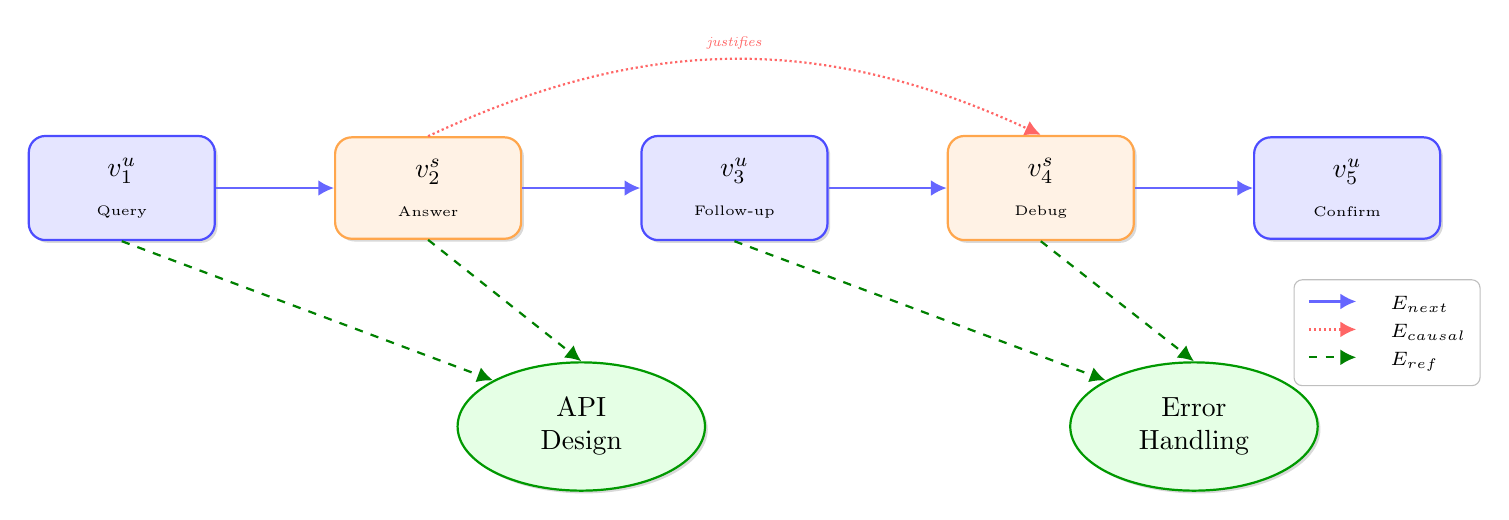
\begin{tikzpicture}[
  node distance=1.8cm and 1.5cm,
  >={Latex[width=2mm,length=2mm]},
  user/.style={
    rectangle, rounded corners=6pt, draw=blue!70, fill=blue!10,
    text width=1.8cm, align=center, inner sep=8pt,
    thick, drop shadow={shadow xshift=1pt, shadow yshift=-1pt, opacity=0.3}
  },
  sys/.style={
    rectangle, rounded corners=6pt, draw=orange!70, fill=orange!10,
    text width=1.8cm, align=center, inner sep=8pt,
    thick, drop shadow={shadow xshift=1pt, shadow yshift=-1pt, opacity=0.3}
  },
  concept/.style={
    ellipse, draw=green!60!black, fill=green!10,
    text width=1.8cm, align=center, inner sep=6pt,
    thick, drop shadow={shadow xshift=1pt, shadow yshift=-1pt, opacity=0.3}
  },
  temporal/.style={->, thick, blue!60},
  causal/.style={->, thick, red!60, densely dotted},
  ref/.style={->, thick, green!50!black, dashed},
]
  % Timeline nodes
  \node[user]    (u1)                     {$v_1^{u}$\\[2pt]{\tiny Query}};
  \node[sys]     (s1) [right=of u1]       {$v_2^{s}$\\[2pt]{\tiny Answer}};
  \node[user]    (u2) [right=of s1]       {$v_3^{u}$\\[2pt]{\tiny Follow-up}};
  \node[sys]     (s2) [right=of u2]       {$v_4^{s}$\\[2pt]{\tiny Debug}};
  \node[user]    (u3) [right=of s2]       {$v_5^{u}$\\[2pt]{\tiny Confirm}};

  % Concept nodes (well below timeline)
  \node[concept] (c1) [below=2.2cm of $(s1)!0.5!(u2)$]  {API\\Design};
  \node[concept] (c2) [below=2.2cm of $(s2)!0.5!(u3)$]  {Error\\Handling};

  % Temporal edges
  \draw[temporal] (u1) -- (s1);
  \draw[temporal] (s1) -- (u2);
  \draw[temporal] (u2) -- (s2);
  \draw[temporal] (s2) -- (u3);

  % Reference edges (vertical, clearly separated)
  \draw[ref] (u1.south) -- (c1.north west);
  \draw[ref] (s1.south) -- (c1.north);
  \draw[ref] (u2.south) -- (c2.north west);
  \draw[ref] (s2.south) -- (c2.north);

  % Causal edge (long-distance arc above)
  \draw[causal] (s1.north) to[bend left=25] node[above, font=\tiny\itshape, pos=0.5] {justifies} (s2.north);

  % Legend
  \node[draw=gray!50, fill=white, rounded corners=3pt, inner sep=5pt,
        font=\scriptsize\sffamily, anchor=north east]
    at ([xshift=0.5cm, yshift=-0.5cm]u3.south east) {
    \begin{tabular}{@{}cl@{}}
      \tikz{\draw[temporal] (0,0) -- (0.6,0);} & $E_{\text{next}}$ \\[2pt]
      \tikz{\draw[causal] (0,0) -- (0.6,0);} & $E_{\text{causal}}$ \\[2pt]
      \tikz{\draw[ref] (0,0) -- (0.6,0);} & $E_{\text{ref}}$ \\
    \end{tabular}
  };
\end{tikzpicture}%
}% end resizebox
\caption{The Trace Episodic DAG. User nodes (blue) and System nodes (orange)
  are connected by temporal edges $E_{\text{next}}$. Reference edges
  $E_{\text{ref}}$ (dashed) anchor episodic events to stable concept nodes
  (green). A causal edge $E_{\text{causal}}$ (dotted) links a justification
  chain across temporal distance. Each node carries an embedding vector
  $\mathbf{e}_v$, timestamp $t_v$, and metadata $m_v$.}
\label{fig:trace-dag}
\end{figure}


% =============================================================================
% Section 3: The Semantic Lookaside Buffer
% =============================================================================
\section{Overcoming Graph Latency: The Semantic Lookaside Buffer}
\label{sec:slb}

While the Trace DAG provides structural fidelity, graph traversal introduces
latency costs that can undermine real-time interaction. Global search over a
growing graph of $N$ nodes incurs $O(\log N)$ complexity per query when using
hierarchical index structures (e.g., HNSW~\cite{malkov2018hnsw}), or $O(N)$
for exhaustive scans. For an agent managing tens of thousands of episodic
nodes across hundreds of sessions, even logarithmic overhead compounds across
the dozens of retrievals required per response generation. To address this, the
Aeon Micro-Graph Kernel introduces the \emph{Semantic Lookaside Buffer}
(SLB), a predictive caching mechanism that exploits a fundamental property of
human-agent dialogue: the locality of semantic topics~\cite{arslan2026aeon}.

\subsection{The Semantic Inertia Hypothesis}

We introduce the concept of \emph{Semantic Inertia} to describe the spatial
correlation inherent in continuous dialogue. In a multi-turn interaction, the
topic vector $\mathbf{q}_i$ at turn $i$ is highly correlated with the topic
vector $\mathbf{q}_{i+1}$ at the subsequent turn:

\begin{equation}
  P\bigl(\text{sim}(\mathbf{q}_{i+1}, \mathbf{q}_i) > \tau\bigr) \approx 1
  \quad \text{for continuous dialogue}
  \label{eq:inertia}
\end{equation}

\noindent where $\text{sim}(\cdot, \cdot)$ denotes cosine similarity and
$\tau$ is a continuity threshold. The intuition is physical: just as a massive
body resists changes to its velocity, a focused conversation resists abrupt
shifts in its semantic trajectory. Topic transitions are overwhelmingly
\emph{incremental} (the next query is a small perturbation of the current
one) rather than \emph{discontinuous}.

This hypothesis is supported empirically. In realistic multi-turn
conversational workloads, consecutive queries share greater than
85\% cosine similarity more than 85\% of the time~\cite{arslan2026aeon}. Abrupt
topic shifts (``hard pivots'') account for fewer than 15\% of transitions, and
even these pivots typically revisit a previously established concept node rather
than introducing an entirely novel topic. This means the ``active
neighborhood'' of the memory graph is highly localized at any given moment: if
the system can predictively pre-fetch this neighborhood, it can bypass the
$O(\log N)$ costs of global search~\cite{arslan2026aeon}.

Research on temporal alignment in language models further supports this
hypothesis. The ``Capacity-Stability Trade-off'' identified in recent work
shows that models can better internalize temporal biases with minimal
``alignment tax''~\cite{dztdpo2025}, validating the use of a dedicated kernel
to manage the stability of the local semantic context while the macro-router
handles global knowledge capacity.

\subsection{Architecture: A Predictive Graph Cache}

The SLB draws its conceptual inspiration from the Translation Lookaside Buffer
(TLB) in traditional operating systems, which accelerates virtual-to-physical
address translation by caching recent mappings. Analogously, the SLB caches the
``active neighborhood'' of the semantic graph to achieve sub-millisecond
retrieval~\cite{arslan2026aeon}.

The SLB is structured as a small, contiguous buffer of $K$ recently accessed
semantic centroids:
\begin{equation}
  B = \{\mathbf{c}_1, \mathbf{c}_2, \ldots, \mathbf{c}_K\}, \quad K \ll N
\end{equation}
where $K$ is tuned to be small enough (typically $K \in [16, 64]$) for rapid
exhaustive comparison. Unlike the global index, which requires hierarchical
tree traversal, the SLB performs a \emph{parallelized similarity comparison}
across all $K$ entries simultaneously. This design makes it a
\emph{software-managed} cache, distinct from traditional OS page caches, that
is optimized specifically for semantic vector operations.

\subsection{Complexity Comparison: $O(K)$ versus $O(\log N)$}

The core complexity advantage is stark. For a query $\mathbf{q}$:

\textbf{SLB lookup (Cache Hit path):}
\begin{equation}
  \text{Cost}_{\text{SLB}}(\mathbf{q}) = O(K) \cdot C_{\text{sim}}
\end{equation}
where $C_{\text{sim}}$ is the cost of a single cosine similarity computation
($O(d)$ for $d$-dimensional vectors). Since $K$ is a small constant
(e.g., 32), this reduces to $O(d)$, effectively constant time
with respect to corpus size $N$.

\textbf{Global index lookup (Cache Miss path):}
\begin{equation}
  \text{Cost}_{\text{Global}}(\mathbf{q}) = O(\log N) \cdot C_{\text{sim}}
  + C_{\text{IO}}
\end{equation}
where $C_{\text{IO}}$ represents the I/O cost of loading index layers from
persistent storage. For HNSW, the logarithmic factor hides a constant
proportional to the number of layers $M$, and each layer hop involves random
access patterns that are cache-unfriendly on modern memory hierarchies.

\textbf{Multi-hop graph reasoning (System 2 path):}
\begin{equation}
  \text{Cost}_{\text{Graph}}(\mathbf{q}) = O(h \cdot b)
\end{equation}
where $h$ is the number of hops and $b$ is the average branching factor. For
complex thematic queries requiring 3--5 hops over a knowledge graph with
branching factor 10--50, this yields $10^3$--$10^5$ node evaluations, orders
of magnitude more expensive than either the SLB or global index path.

The SLB's $O(K)$ cost is \emph{independent} of corpus size, making it
asymptotically optimal for the common case of high semantic locality. When the
Semantic Inertia hypothesis holds (Equation~\ref{eq:inertia}), the SLB
intercepts the vast majority of queries before they ever reach the global
index, amortizing the expensive $O(\log N)$ path over the rare cache-miss
events.

\subsection{The Speculative Fetch Algorithm}

The lookup procedure proceeds as follows: given a query
$\mathbf{q} \in \mathbb{R}^d$, the system computes the similarity
$s_j = \text{sim}(\mathbf{q}, \mathbf{c}_j)$ for every cached centroid
$\mathbf{c}_j \in B$, selects the best match
$s_{\text{best}} = \max_j s_j$, and evaluates against the hit threshold
$\tau_{\text{hit}}$:

\begin{itemize}
  \item If $s_{\text{best}} > \tau_{\text{hit}}$ (typically 0.85): a
    \textbf{Cache Hit} is declared, and the system returns the direct pointer to
    the corresponding Atlas graph node, bypassing the global index
    entirely~\cite{arslan2026aeon}.
  \item If $s_{\text{best}} \leq \tau_{\text{hit}}$: a \textbf{Cache Miss}
    triggers an authoritative fallback to the full Atlas index, and the result
    populates the SLB via a Least Recently Used (LRU) eviction
    policy~\cite{arslan2026aeon}.
\end{itemize}

Algorithm~\ref{alg:slb} formalizes this speculative fetch procedure.
In production environments, the buffer $B$ requires a thread-safe ring buffer
or read-copy-update (RCU) mechanism to prevent read-write race conditions
during the \textsc{AsyncPrefetch} routine, and $\tau_{\text{hit}}$ is
treated as an empirically tuned hyperparameter.

\begin{algorithm}[t]
\caption{Semantic Lookaside Buffer: Speculative Fetch}
\label{alg:slb}
\begin{algorithmic}[1]
\Require Query vector $\mathbf{q}$, Buffer $B = \{\mathbf{c}_1, \ldots, \mathbf{c}_K\}$, Threshold $\tau_{\text{hit}}$
\Ensure Retrieved node pointer $p^*$
\State $s_{\text{best}} \gets -\infty$, $j^* \gets \text{null}$
\For{$j = 1$ to $K$} \Comment{Parallelized comparison}
    \State $s_j \gets \text{sim}(\mathbf{q}, \mathbf{c}_j)$
    \If{$s_j > s_{\text{best}}$}
        \State $s_{\text{best}} \gets s_j$, $j^* \gets j$
    \EndIf
\EndFor
\If{$s_{\text{best}} > \tau_{\text{hit}}$} \Comment{Cache Hit}
    \State $p^* \gets \text{pointer}(\mathbf{c}_{j^*})$
    \State \Call{AsyncPrefetch}{children of $p^*$} \Comment{Speculative loading}
    \State \Return $p^*$
\Else \Comment{Cache Miss}
    \State $p^* \gets \text{AtlasFullSearch}(\mathbf{q})$
    \State $\textsc{LRU-Insert}(B,\; \mathbf{q},\; p^*)$
    \State \Return $p^*$
\EndIf
\end{algorithmic}
\end{algorithm}

\subsection{Asynchronous Prefetching and Hierarchical Loading}

A key property of the SLB is its ability to perform \emph{asynchronous
prefetching} during natural pauses in user interaction (typing delays, reading
time, or inter-turn gaps). When a Cache Hit occurs on node $p^*$ at depth $d$ in
the Atlas hierarchy, the system speculatively loads the children of $p^*$ from
the persistent index into the SLB~\cite{arslan2026aeon}. This leverages the
hierarchical topology of the Atlas spatial index: if a user is querying a
sub-topic (e.g., ``vector database benchmarks'') and the SLB hits on the
broader ``Database'' concept node $c_{\text{db}}$, the system proactively stages
the ``Vector ANN'' and ``Query Optimization'' child nodes into the buffer:
\begin{equation}
  B' = B \cup \{c \mid (c_{\text{db}}, c) \in E_{\text{Atlas}}\}
\end{equation}
This effectively pipelines the semantic navigation, hiding the memory latency
of the global graph behind the user's cognitive processing time.

Empirical evaluation on realistic conversational workloads demonstrates that the
SLB achieves hit rates exceeding 85\%, reducing the effective retrieval latency
by approximately 6$\times$ compared to full graph
traversal~\cite{arslan2026aeon}. This aligns with findings from the
knowledge-graph-enhanced semantic cache literature, which reports significant
latency improvements from caching semantically similar
prompts~\cite{kgcache2024}, and with hierarchical memory architectures that
show top-down routing reduces search complexity from exhaustive enumeration to
targeted traversal~\cite{hmem2025}.


% =============================================================================
% Section 4: Cognitive Routing and Enterprise Graph Integration
% =============================================================================
\section{Cognitive Routing and Enterprise Graph Integration}
\label{sec:routing}

While the Micro-Graph Kernel manages the episodic state (Layer~1), the
Macro-Graph Router (PandoraLM) handles the ``System~2'' reasoning over global
structures (Layer~2). This dual-process routing ensures that the agent can
navigate complex relational data and enforce enterprise-grade security without
compromising interaction speed.

\subsection{Dual-Process Strategy Selection}

PandoraLM functions as a meta-cognitive layer that analyzes query
characteristics to determine the optimal reasoning
depth~\cite{cognitiverouting2025}. Inspired by Kahneman's dual-process theory
of cognition~\cite{kahneman2011}, the router classifies every incoming query
into one of four categories and dispatches it along the appropriate execution
path:

\begin{itemize}
  \item \textbf{System~1 (Fast, Intuitive):} Queries classified as
    \textsc{factual} (direct lookups, definitions, simple
    retrievals) are routed to a high-speed vector store. This path optimizes
    for latency, returning results through approximate nearest neighbor
    search over dense embeddings. System~1 processing mirrors the automatic,
    low-effort cognitive responses described by Kahneman, where the cost of
    deliberation would exceed the value of the answer.

  \item \textbf{System~2 (Slow, Deliberate):} Queries classified as
    \textsc{thematic} or \textsc{research} (those requiring relational
    reasoning, cross-document synthesis, or multi-hop traversal) are routed
    to a knowledge graph store. This path employs Cypher
    queries over a Neo4j graph database, enabling the agent to reason about
    entity relationships, temporal evolution, and thematic
    conflicts~\cite{edge2024graphrag}. System~2 processing corresponds to
    the effortful, analytical cognition reserved for problems that demand
    structural understanding.

  \item \textbf{Code Path:} Queries classified as \textsc{code} (those
    involving source code understanding, debugging, or implementation) are
    dispatched to the Code Brain pipeline (Section~\ref{sec:codebrain}),
    which operates over structural AST representations rather than text
    chunks.
\end{itemize}

Preliminary internal evaluation of the PandoraLM implementation yielded up
to a 70\% reduction in API inference costs compared to an always-on reasoning
model baseline.
The dual-process framing also aligns with
Reasoning RAG architectures that distinguish between predefined (System~1) and
agentic (System~2) reasoning modes~\cite{sysrag2025}, and with research on
routing collapse prevention that addresses the risk of underutilizing
specialized retrieval pipelines~\cite{equirouter2026}.

\subsection{Structural Code Representation: The Code Brain}
\label{sec:codebrain}

Standard text chunking is a primary source of Vector Haze in coding tasks.
Traditional methods break code into fixed-size segments, often severing a
function signature from its body or an import statement from its usage
site~\cite{cast2025}. PandoraLM addresses this through AST-aware structural
chunking.

Using the Tree-sitter parser, source code is parsed into a hierarchical tree of
typed syntax nodes (e.g., \texttt{FunctionDefinition},
\texttt{ClassDeclaration}). A recursive ``split-then-merge'' algorithm ensures
that code is divided into segments that respect program logic and preserve
structural boundaries~\cite{cast2025}. Each chunk retains ``breadcrumb
context'' (metadata headers specifying its parent class, inherited methods, and
invoked dependencies) so that when a snippet is retrieved, the LLM understands
its position within the larger codebase architecture.

These structural nodes are then mapped into the knowledge graph using typed
relationships:

\begin{itemize}
  \item \texttt{CONTAINS}: A module contains classes and functions.
  \item \texttt{CALLS}: Function $A$ invokes function $B$.
  \item \texttt{INHERITS}: Class $C$ extends class $D$.
  \item \texttt{IMPORTS}: Module $X$ depends on module $Y$.
  \item \texttt{HAS\_METHOD}: Class $C$ defines method $m$.
\end{itemize}

\noindent Empirical evaluation of AST-based retrieval shows significant gains,
with a 5.5-point improvement on code retrieval benchmarks compared to
line-based chunking~\cite{cast2025}.

\subsubsection{Failure Scenario: Polymorphic Method Resolution}

To illustrate why structural graph retrieval is necessary, consider a
concrete failure scenario involving polymorphic inheritance.

\textbf{Setup.} A large enterprise codebase contains a base class
\texttt{PaymentProcessor} with a method \texttt{authorize()}, and two
subclasses: \texttt{CreditCardProcessor} (which overrides
\texttt{authorize()} to add fraud-check logic) and \texttt{CryptoProcessor}
(which overrides \texttt{authorize()} to call a blockchain validation
service). A developer asks the agent: ``\emph{Why does
\texttt{authorize()} sometimes call the fraud-check service and sometimes
the blockchain service?}''

\textbf{Flat RAG Failure.} A traditional text-chunking pipeline indexes
each method body as an independent text chunk. The query ``authorize()''
returns the three highest-similarity chunks: (1) \texttt{PaymentProcessor.authorize()}
(the base method), (2) \texttt{CreditCardProcessor.authorize()}, and
(3) an unrelated \texttt{AuthService.authorize\_user()} from a different
module that happens to share similar vocabulary. The flat retriever
\emph{cannot} represent the inheritance relationship, so it presents
three disconnected code fragments. The LLM, seeing no structural link
between them, may hallucinate an incorrect explanation or fail to
identify that \texttt{CryptoProcessor} even exists, because its
\texttt{authorize()} method is ranked below the irrelevant
\texttt{AuthService}.

\textbf{AST Graph Resolution.} The Code Brain pipeline parses the
codebase into typed AST nodes and maps them into the knowledge graph.
Upon receiving the query, the system:
\begin{enumerate}
  \item Retrieves the node for \texttt{PaymentProcessor.authorize()} via
    semantic search.
  \item Traverses \texttt{INHERITS} edges to discover all subclasses:
    \texttt{CreditCardProcessor} and \texttt{CryptoProcessor}.
  \item For each subclass, traverses \texttt{HAS\_METHOD} edges to find
    their respective \texttt{authorize()} overrides.
  \item Traverses \texttt{CALLS} edges from each override to discover the
    downstream services: \texttt{FraudCheckService} and
    \texttt{BlockchainValidator}.
\end{enumerate}

The result is a complete, structurally verified inheritance tree with full
call-chain context. The LLM receives \emph{all} relevant methods in their
hierarchical relationship, enabling a precise explanation of polymorphic
dispatch. This multi-hop traversal (\texttt{INHERITS} $\to$
\texttt{HAS\_METHOD} $\to$ \texttt{CALLS}) is computationally intractable
to reconstruct in a flat vector store without maintaining costly, out-of-band
relational indices.

\subsection{ReBAC Security: Eliminating TOCTOU Vulnerabilities}
\label{sec:rebac}

In enterprise environments, the Macro-Graph also serves as the enforcement
layer for \emph{Relationship-Based Access Control} (ReBAC). Data is partitioned
into hierarchical \textbf{Knowledge Layers} (\textsc{system},
\textsc{organization}, \textsc{team}, and \textsc{user}), each representing a
scope of visibility and control.

\subsubsection{The TOCTOU Problem in Standard RAG}

Standard RAG pipelines suffer from a subtle but critical
\emph{Time-of-Check to Time-of-Use} (TOCTOU) vulnerability. The typical
pattern is:
\begin{enumerate}
  \item The system checks the user's permissions (Time-of-Check).
  \item The retriever queries the vector store and returns candidate
    documents.
  \item A post-hoc filter removes documents the user is not authorized
    to see (Time-of-Use).
\end{enumerate}
Between steps 1 and 3, the unauthorized documents have already been
\emph{loaded into memory}, their embeddings have participated in similarity
calculations, and, critically, they may have influenced the ranking of
authorized documents. In adversarial settings, carefully crafted prompts can
exploit this window to extract information about the \emph{existence} of
unauthorized documents (via ranking perturbation attacks) even if their
content is filtered. The unauthorized data has already entered the
reasoning context before the filter is applied.

\subsubsection{Deterministic Pre-Filtering via Layer Injection}

PandoraLM systematically mitigates this vulnerability through
\emph{deterministic pre-filtering}. Every incoming request carries an
\texttt{X-Pandora-Layer-ID} header derived from the user's Identity
Passport (e.g., Keycloak group memberships). This header is not merely
a metadata annotation; it is injected directly into the Cypher execution
plan as a \texttt{WHERE} clause constraint:

\begin{verbatim}
MATCH (n:KnowledgeNode)
WHERE n.layer_id IN $authorized_layers
AND   n.embedding <-> $query_vec < $threshold
RETURN n
\end{verbatim}

The \texttt{layer\_id IN \$authorized\_layers} constraint is evaluated
by the Neo4j query planner \emph{before} any embedding similarity
calculations occur. Unauthorized nodes are physically excluded from the
traversal set: they are never loaded, never compared, and never
ranked. This transforms the security model from \emph{filter-after-retrieval}
(TOCTOU-vulnerable) to \emph{restrict-before-traversal}
(TOCTOU-resistant). Assuming the database query planner strictly enforces
pre-filtering prior to vector index traversal, this deterministic approach
minimizes the window of time during which unauthorized data can influence
reasoning pipelines, though timing side-channels remain an open challenge.

Figure~\ref{fig:routing} illustrates the cognitive routing architecture and its
interaction with the underlying Aeon kernel.

% ---- FIGURE 2: Dual-Process Routing Flowchart ----
\begin{figure}[t]
\centering
\resizebox{\textwidth}{!}{%
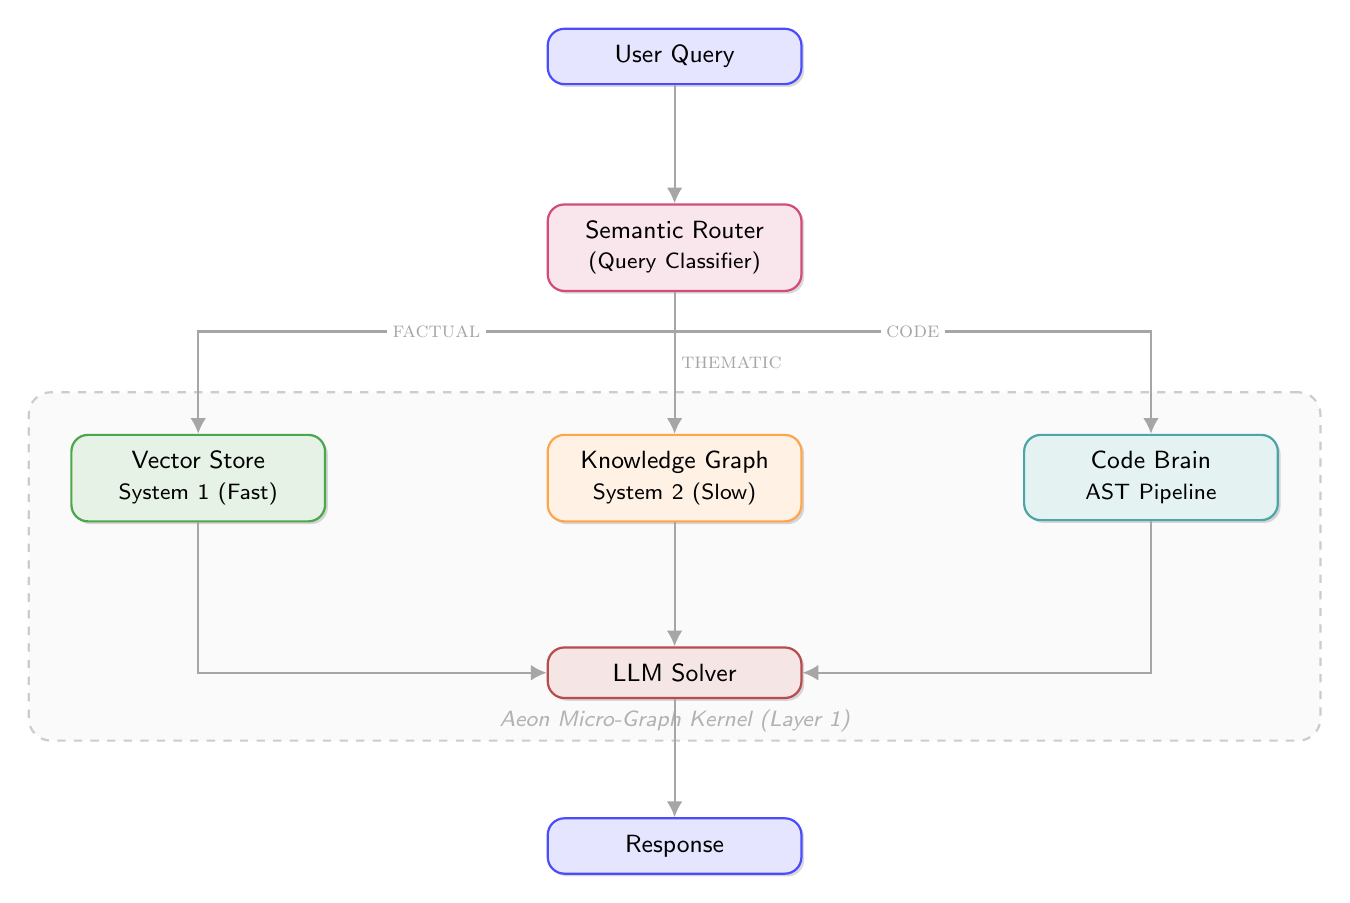
\begin{tikzpicture}[
  node distance=1.5cm and 2.0cm,
  >={Latex[width=2mm,length=2mm]},
  process/.style={
    rectangle, rounded corners=6pt, draw=#1!70, fill=#1!10,
    text width=2.8cm, align=center, inner sep=6pt,
    thick, drop shadow={shadow xshift=1pt, shadow yshift=-1pt, opacity=0.3},
    font=\small\sffamily
  },
  process/.default=gray,
  routerbox/.style={
    rectangle, rounded corners=6pt, draw=purple!70, fill=purple!10,
    text width=2.8cm, align=center, inner sep=6pt,
    thick, drop shadow={shadow xshift=1pt, shadow yshift=-1pt, opacity=0.3},
    font=\small\sffamily
  },
  arrow/.style={->, thick, gray!70},
  elabel/.style={font=\footnotesize\sffamily, fill=white, inner sep=2pt},
]
  % Row 1: Query
  \node[process=blue] (query) {User Query};

  % Row 2: Router
  \node[routerbox] (router) [below=of query] {Semantic Router\\{\footnotesize (Query Classifier)}};

  % Row 3: Three retrieval paths (well-spaced)
  \node[process=green!50!black] (vec) [below left=1.8cm and 2.8cm of router] {Vector Store\\{\footnotesize System 1 (Fast)}};
  \node[process=orange] (graph) [below=1.8cm of router] {Knowledge Graph\\{\footnotesize System 2 (Slow)}};
  \node[process=teal] (code) [below right=1.8cm and 2.8cm of router] {Code Brain\\{\footnotesize AST Pipeline}};

  % Row 4: LLM Solver
  \node[process=red!60!black] (solver) [below=4.5cm of router] {LLM Solver};

  % Row 5: Response
  \node[process=blue] (response) [below=of solver] {Response};

  % Kernel background
  \begin{scope}[on background layer]
    \node[
      rectangle, rounded corners=8pt, draw=gray!40, fill=gray!4,
      dashed, thick, inner sep=15pt,
      fit=(vec)(graph)(code)(solver)
    ] (kernel) {};
    \node[font=\footnotesize\sffamily\itshape, gray!60, anchor=south]
      at (kernel.south) {Aeon Micro-Graph Kernel (Layer 1)};
  \end{scope}

  % Arrows: Query -> Router
  \draw[arrow] (query) -- (router);

  % Arrows: Router -> Retrieval (using orthogonal routing)
  \draw[arrow] (router.south) -- ++(0,-0.5) -| (vec.north)
    node[elabel, pos=0.25] {\textsc{factual}};
  \draw[arrow] (router) -- (graph)
    node[elabel, midway, right] {\textsc{thematic}};
  \draw[arrow] (router.south) -- ++(0,-0.5) -| (code.north)
    node[elabel, pos=0.25] {\textsc{code}};

  % Arrows: Retrieval -> Solver (orthogonal, no crossing)
  \draw[arrow] (vec.south) |- (solver.west);
  \draw[arrow] (graph) -- (solver);
  \draw[arrow] (code.south) |- (solver.east);

  % Arrows: Solver -> Response
  \draw[arrow] (solver) -- (response);
\end{tikzpicture}%
}% end resizebox
\caption{PandoraLM Cognitive Routing Architecture. The Semantic Router
  classifies incoming queries and dispatches them to System~1 (Vector Store),
  System~2 (Knowledge Graph), or the Code Brain (AST). All paths converge at
  the LLM Solver using orthogonal routing. The dashed boundary indicates the
  Aeon Micro-Graph Kernel underlying all retrieval operations.}
\label{fig:routing}
\end{figure}


% =============================================================================
% Section 5: Discussion
% =============================================================================
\section{Discussion: Synergizing the Kernel and the Router}
\label{sec:discussion}

The fundamental architectural challenge of a dual-layer cognitive OS is the
tension between the high-speed, verbose episodic DAG (Layer~1) and the
consolidated, global knowledge graph (Layer~2). If every conversation turn were
directly injected into the global knowledge graph, it would quickly become
cluttered with transient noise, leading to retrieval degradation. Conversely, if
the episodic DAG remains isolated, the agent cannot build cumulative,
cross-session understanding. This paper proposes a theoretical \emph{Memory
Consolidation} process, a ``Dreaming'' phase, as the bridge between
layers~\cite{arslan2026aeon}. In this framework, \emph{Memory Consolidation}
refers to the biological\slash system \emph{process} of migrating transient
episodic data from the Trace DAG into long-term storage, whereas the
\emph{Memory Palace} denotes the \emph{spatial Atlas index} where consolidated
long-term episodic concepts permanently reside. While Layer~1 and Layer~2
have been implemented as independent reference systems, their real-time
fusion via the Dreaming consolidation pipeline remains an active area of
architectural research.

\subsection{The Serialization Challenge}

In the current architecture, Layer~1 and Layer~2 operate independently. The
Aeon Micro-Graph Kernel manages within-session episodic memory with
sub-millisecond responsiveness, while PandoraLM's knowledge graph handles
cross-session structural reasoning. Bridging these layers in real-time creates
a serialization bottleneck: the raw, verbose trace data generated during
high-speed interaction cannot be efficiently transmitted to the distributed
graph router without incurring prohibitive overhead. A single 30-minute
interaction session may generate hundreds of episodic nodes with full
embedding payloads, metadata records, and edge sets, far too much data to
inject into a production Neo4j instance synchronously without degrading
query performance for concurrent users.

The Dreaming process solves this by \emph{decoupling the ingestion of
experience from the consolidation of knowledge}. While the agent is ``awake''
and interacting, the kernel stores every raw detail in the episodic DAG. During
idle time (between sessions or during scheduled maintenance
windows) the Dreaming background process activates to transform fragile
episodic traces into stable, long-term semantic knowledge within the Memory
Palace~\cite{lmsleep2025}.

\subsection{The Sleep-Inspired Consolidation Pipeline}

The consolidation process mirrors the biological interaction between the
hippocampus and the neocortex, where memories are replayed and integrated into
the existing knowledge network. Table~\ref{tab:consolidation} outlines the
four-stage pipeline.

\begin{table}[t]
  \caption{Memory Consolidation Pipeline}
  \label{tab:consolidation}
  \begin{tabular}{lll}
    \toprule
    \textbf{Stage} & \textbf{Biological Parallel} & \textbf{Implementation} \\
    \midrule
    Clustering    & Failure Analysis       & LLM-based grouping \\
    Abstraction   & Gist Extraction        & Candidate rule synthesis \\
    Active Dream  & Counterfactual Test    & Scenario simulation \\
    Integration   & Synaptic Adjustment    & KG commit + prune \\
    \bottomrule
  \end{tabular}
\end{table}

\textbf{Clustering.} The first stage groups related episodic traces; for
example, clustering all debugging sessions that involved the same API endpoint
or all conversations that referenced a particular architectural decision. The
clustering uses the reference edges $E_{\text{ref}}$: nodes sharing common
concept anchors $\mathcal{A}(v_i) \cap \mathcal{A}(v_j) \neq \emptyset$ are
candidates for the same cluster.

\textbf{Abstraction.} From each cluster, the system synthesizes ``candidate
rules,'' generalized knowledge statements that abstract away the specific
details of individual episodes. A cluster of five debugging conversations about
null pointer exceptions in the authentication module, for instance, might yield
the candidate rule: ``The OAuth token refresh path does not handle concurrent
requests safely.''

\textbf{Active Dreaming.} This stage goes beyond passive replay. Using the
LLM, the system generates counterfactual simulations: ``If I apply this new
rule to a different but related situation, does it still
hold?''~\cite{lmsleep2025}. Only rules that survive synthetic verification
in a sandboxed environment proceed to the next stage.

\textbf{Integration.} Verified rules are committed to the PandoraLM knowledge
graph as new entity nodes with structural edges linking them to relevant
concepts, projects, and teams. These consolidated nodes reside permanently
within the Memory Palace spatial index.

\subsection{Graph Pruning: Deciding What to Forget}

After integration, the system must decide which episodic nodes to prune.
Aggressive pruning risks losing causal navigability; insufficient pruning
allows unbounded graph growth. We define a pruning eligibility function
$\phi(v)$ that determines whether an episodic node $v$ can safely transition
to \emph{dormant} status:

\begin{equation}
  \phi(v) =
  \begin{cases}
    \text{\textsc{dormant}} & \text{if } \forall\, (v, c) \in E_{\text{ref}} :
      c \in V_{\text{committed}} \\
      & \quad \land\; |\{(v, w) \in E_{\text{causal}}\}| = 0 \\
      & \quad \land\; \text{age}(v) > T_{\text{decay}} \\[4pt]
    \text{\textsc{active}} & \text{otherwise}
  \end{cases}
\end{equation}

A node is eligible for dormancy if and only if: (1) all concept nodes it
references have already been committed to the global KG
($V_{\text{committed}}$), meaning no information is lost; (2) it has no
outgoing causal edges, meaning no downstream decisions depend on it as a
premise; and (3) it has exceeded the decay threshold $T_{\text{decay}}$,
ensuring recent nodes remain accessible regardless of their structural
properties.

\subsubsection{Pruning Invariants}

Two graph invariants must be preserved after pruning to guarantee continued
correctness of traversal operations:

\textbf{Invariant 1: Temporal Chain Integrity.} If a node $v_i$ is pruned,
the temporal edges $E_{\text{next}}$ must be repaired to maintain a connected
backbone:
\begin{equation}
  \text{If } v_i \text{ is pruned and }
  (v_{i-1}, v_i), (v_i, v_{i+1}) \in E_{\text{next}},
  \text{ then add } (v_{i-1}, v_{i+1}) \text{ to } E_{\text{next}}
\end{equation}
This ``edge contraction'' preserves the total ordering of the timeline,
ensuring that backtracking via $E_{\text{next}}^{-1}$ never encounters a
broken chain.

\textbf{Invariant 2: Causal Ancestor Preservation.} No node $v$ may be
pruned if there exists any active node $w$ such that
$(v, w) \in E_{\text{causal}}$. This ensures that every active decision
retains its full justification chain, enabling root-cause analysis at any
time.

Dormant nodes are not deleted; they are moved to a compressed archival store
with their embeddings and metadata intact. They can be ``reawakened'' if a
future query strongly matches their embedding (i.e., a Cache Miss that
resolves to an archival node), at which point they are restored to the active
Trace and their edges are rehydrated.

\subsection{Strategic Benefits}

This synergy yields three core advantages:

\begin{itemize}
  \item \textbf{Knowledge Retention:} Stress tests on self-modifying memory
    consolidation report 95\% knowledge retention after 500 episodic
    cycles, effectively mitigating catastrophic
    forgetting~\cite{lmsleep2025}.
  \item \textbf{Storage Efficiency:} Consolidation reduces storage growth by
    abstracting verbose transcripts into concise gists, allowing raw details
    to slip into dormancy unless specifically
    recalled~\cite{zhang2026continuum}.
  \item \textbf{Associative Routing:} By building structural edges between
    abstracted nodes (linking a technology to a project and its
    team) the system enables ``spreading activation'': the ability to
    perform multi-hop recall even when exact query terms are
    absent~\cite{zhang2026continuum}.
\end{itemize}


% =============================================================================
% Section 6: Conclusion and Open Questions
% =============================================================================
\section{Conclusion and Open Questions}
\label{sec:conclusion}

This paper has presented a dual-layer Cognitive Operating System that addresses
the Vector Haze problem by replacing flat vector retrieval with structured,
navigable graph topologies. Layer~1 (the Aeon Micro-Graph Kernel) formalizes
episodic memory as a neuro-symbolic DAG with formally defined temporal, causal,
and referential edge families (Equations 3--6), providing $O(k)$ exact causal
backtracking versus $O(\log N)$ approximate semantic retrieval. The Semantic
Lookaside Buffer achieves $O(K)$ retrieval complexity through predictive graph
caching, exploiting the Semantic Inertia of continuous dialogue to intercept
85\%+ of queries before they reach the global index.

Layer~2 (the PandoraLM Macro-Graph Router) implements Kahneman-inspired
cognitive routing that eliminates computational waste through query
classification, AST-aware code representation that resolves polymorphic
inheritance chains impossible to navigate via flat chunking, and deterministic
ReBAC security that eliminates TOCTOU vulnerabilities by physically excluding
unauthorized nodes from the traversal set before any similarity computation.
The proposed Dreaming consolidation process bridges the two layers through a
biologically inspired four-stage pipeline with formally defined pruning
invariants (temporal chain integrity and causal ancestor preservation) that
guarantee correctness under graph contraction.

Three open questions warrant collaborative investigation:

\begin{enumerate}
  \item \textbf{Symbolic Edge Maintenance Under Neural Concept Drift.}
    The Trace DAG's symbolic edges ($E_{\text{causal}}$, $E_{\text{ref}}$) are
    defined relative to specific neural embedding models. When the underlying
    embedding model is upgraded or fine-tuned, the geometric relationships
    between node vectors shift, potentially invalidating reference edges that
    were assigned under the previous space's similarity metric (Equation~5).
    How should the system detect and repair stale symbolic edges without full
    $O(|V| \times |V_{\text{concept}}|)$ re-computation of the reference
    edge set?

  \item \textbf{Dynamic Pruning of Episodic DAGs.}
    The pruning eligibility function $\phi(v)$ (Equation~15) provides a
    conservative baseline: nodes are only pruned when all their semantic
    content has been committed to the global KG. However, in
    high-throughput environments where an agent processes thousands of
    turns per day, even this conservative policy may leave an unmanageable
    residual graph. What relaxed invariants can be defined that allow
    more aggressive pruning (e.g., pruning causal ancestors if their
    \emph{effects} have been independently verified) while bounding the
    probability of information loss?

  \item \textbf{Vector Dimensionality and Multi-Modality.}
    Current spatial memory kernels often hardcode embedding dimensions
    (e.g., $d=768$ for BERT-family models). As agent architectures
    increasingly integrate heterogeneous data sources, a critical question
    arises: how can graph-based memory OS kernels dynamically adapt to
    variable-length or multi-modal embeddings (e.g., integrating
    1536-dimensional text embeddings with high-dimensional CLIP image
    embeddings) within the same episodic DAG, without incurring catastrophic
    spatial fragmentation of the Atlas index or prohibitive re-indexing costs
    across the Memory Palace?
\end{enumerate}

The workshop community is invited to engage with these questions and contribute
toward a scalable, principled framework for neuro-symbolic agent memory.


% =============================================================================
% Code Availability
% =============================================================================
\subsection*{Code Availability}

Reference implementations of the architectures discussed in this paper are
available as open-source repositories. The Macro-Graph Router (PandoraLM) can
be accessed at \url{https://github.com/mustafarslan/pandoralm}, and the
Micro-Graph Kernel (Aeon) at \url{https://github.com/mustafarslan/aeon}.
Empirical metrics reported for the reference implementations (e.g., 70\% cost
reduction, 85\% cache hit rates) were derived from internal benchmarks on
simulated multi-turn technical workloads using local LLMs (e.g., 1B parameter
router, 8B parameter solver). Full methodological details are available within
the respective repositories.


% =============================================================================
% Bibliography
% =============================================================================
\bibliography{references}

\end{document}
